\section{Separate changed-background sensitivity}
\label{app:background}

\paragraph{Design and target.}
After the primary fixed-background panel, a bounded supplementary arm used ACSIncome and Diabetes with all three previously fitted models. It retained the first twelve main inputs in their original random order and did not refit models or redraw explained inputs. For each fitted cell, one background of 8 and one of 128 training rows were drawn without replacement, with recorded SeedSequence inputs beginning with 60793. Each game was exactly enumerated, and each estimator ran twenty independent seeds at the dataset's middle nominal budget (ACS 256; Diabetes 64). Seeds, training/background/source-input IDs, signatures, vectors and costs are retained in \texttt{results/background/}. The arm contains 144 changed-game exact references and 5,760 stochastic calls across six fitted cells, separately audited and aggregated under \texttt{results/background\_sensitivity/}.

\paragraph{Two comparisons.}
Estimation accuracy compares a stochastic vector with the exact reference for its own changed background, using the same primary criterion and its new reference norm. Target sensitivity instead compares that changed exact vector with the original B32 exact vector on the same input. For the latter comparison, normalized L1 uses the B32 norm and floor; B32 is a comparison target, not population truth. The stored reference-shift columns named error or match describe differences between two exact games. These are not causal errors or extra primary estimator replicates. Instance-cluster uncertainty uses twelve inputs, preserving repeats for the stochastic comparison; all-success displayed intervals are $[.6080,1]$, rather than zero-width bootstrap endpoints.

\paragraph{Measured target shifts and stochastic accuracy.}
For B8, mean normalized exact-target shifts from B32 range from $.2914$ for ACS forest to $.5364$ for Diabetes histogram boosting; for B128 they range from $.1247$ to $.2606$ on those same fitted cells. ACS logistic B8 has mean shift $.4977$, interval $[.4335,.5641]$, while both stochastic estimators have observed success $1$ against that B8 target. The most salient exact feature changes on 4/12 of those inputs: top-one agreement $.6667$, interval $[.4167,.9167]$. Thus high estimation accuracy for one game does not establish invariance to a different background choice.

Across changed-game conditions, observed primary success ranges from $.9083$ to $1$. The lowest condition is Diabetes histogram boosting with permutation at B8: $.9083$ $[.8125,.9792]$. B128 condition means are $.9958$ or $1$. Full signed-selection, absolute-shift and top-one outcomes are supplied, with all twelve cases retained. Only one row sample per size is used, so size and resampling effects are confounded. This arm supports conditional target sensitivity for the tested draws, not a pure-size effect, population background variance, German Credit generalization or model-retraining robustness.

\paragraph{Cost and software notices.}
The timed pilot preceded expansion, with 96 stochastic calls and 24 exact targets, and projected 17.44 CPU minutes (26.16 with its safety allowance). Full supplementary cell-phase timers record 466.053 CPU seconds, excluding initial imports and bundle/data loading. Sampled resource-reported job costs are retained separately and can undershoot these phase timers; neither scope is an exact all-inclusive CPU total. All 18 captured first-import Matplotlib colormap-deprecation notices are retained with their disposition; no numerical warning or failed attempt was recorded. The background arm does not inherit the primary panel's zero-warning count.

\paragraph{Audit and reproduction.}
The supplied audit verifies the full source/grid/seeds, training-only background draws, original input identity, main comparison reference, exact endpoints/efficiency and Kernel design rank. Its seeds are unique within the supplementary arm and disjoint from primary seeds. Audit/reaggregation uses the shipped checkpoints without a fitted bundle. To rerun explanations, first regenerate main models into a fresh output root, then run \texttt{analysis/scripts/run\_background\_queue.py} against that root and \texttt{analysis/scripts/aggregate\_background.py}; exact integrated commands are in \texttt{analysis/README.md}. The raw main checkpoints intentionally omit fitted joblib bundles, so requesting resume against them is not the regeneration route.

\clearpage
\input{tables/background_compute.tex}
\clearpage
\begin{figure}[tb]
\centering
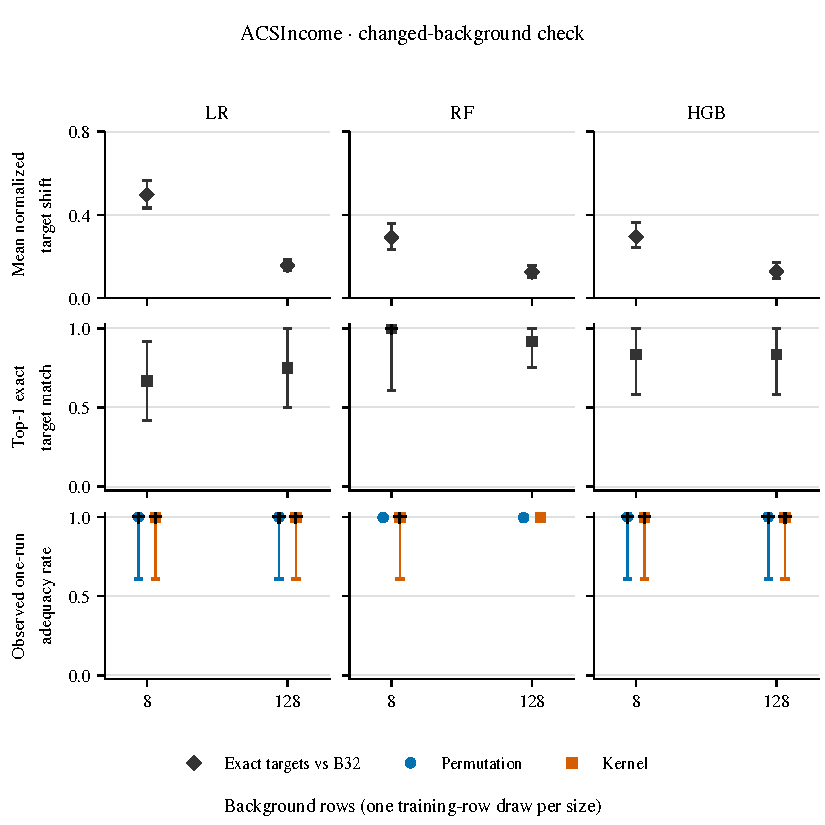
\includegraphics[width=\linewidth]{figures/background_sensitivity_acs.pdf}
\caption[Changed-background target sensitivity and own-target accuracy.]{Changed-background sensitivity for ACSIncome. Top: exact changed-game attribution versus the main B32 exact attribution, using L1 difference/max(B32 attribution L1,0.01). Middle: fraction of inputs with the same most salient absolute-attribution feature under those two exact targets (stable raw-index tie order). These measure a target shift, not estimator error; B32 is a comparison target, not population truth. Bottom: stochastic accuracy against each changed game's own exact target, requiring normalized L1 <=0.20 and signed top-3 overlap >=2/3 with floor 0.01. Both estimators use the middle requested budget (256); actual work is not equated. The same 12 main inputs and fitted models are retained, with 20 independent runs per input/estimator/background; exact target comparisons use one value per input. Bars are supplied pointwise 95\% instance-cluster percentile intervals, conditional on each fitted model and each single background draw; black plus marks identify supplied two-sided Hoeffding boundary intervals for all-success panels. No >=0.95 population or individual certificate follows. Whole-row empirical interventional integration uses positive-class probability and grouped raw features. Size and selected training rows change together; one draw per size cannot identify a pure-size effect or background-population variance. These calls are separate from fixed-B32 main repetitions.
}
\label{fig:background-acs}
\end{figure}
\clearpage
\begin{figure}[tb]
\centering
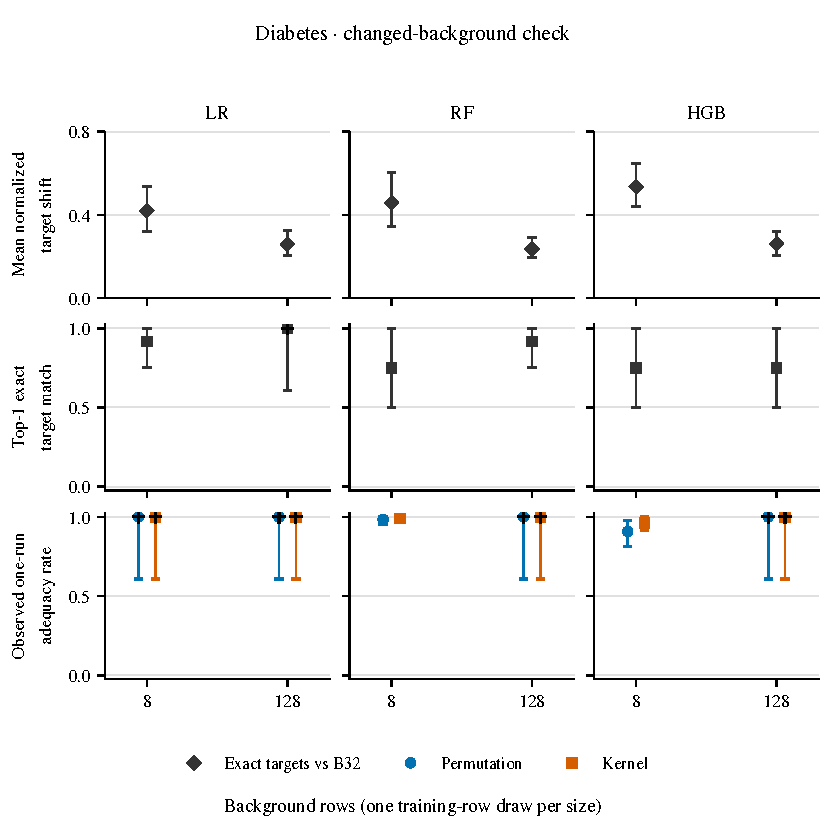
\includegraphics[width=\linewidth]{figures/background_sensitivity_diabetes.pdf}
\caption[Changed-background target sensitivity and own-target accuracy.]{Changed-background sensitivity for Diabetes. Top: exact changed-game attribution versus the main B32 exact attribution, using L1 difference/max(B32 attribution L1,0.01). Middle: fraction of inputs with the same most salient absolute-attribution feature under those two exact targets (stable raw-index tie order). These measure a target shift, not estimator error; B32 is a comparison target, not population truth. Bottom: stochastic accuracy against each changed game's own exact target, requiring normalized L1 <=0.20 and signed top-3 overlap >=2/3 with floor 0.01. Both estimators use the middle requested budget (64); actual work is not equated. The same 12 main inputs and fitted models are retained, with 20 independent runs per input/estimator/background; exact target comparisons use one value per input. Bars are supplied pointwise 95\% instance-cluster percentile intervals, conditional on each fitted model and each single background draw; black plus marks identify supplied two-sided Hoeffding boundary intervals for all-success panels. No >=0.95 population or individual certificate follows. Whole-row empirical interventional integration uses positive-class probability and grouped raw features. Size and selected training rows change together; one draw per size cannot identify a pure-size effect or background-population variance. These calls are separate from fixed-B32 main repetitions.
}
\label{fig:background-diabetes}
\end{figure}
\clearpage
